\phantomsection
\addcontentsline{toc}{chapter}{Abbildungsverzeichniss}

\listoffigures




\phantomsection
\addcontentsline{toc}{chapter}{Literaturverzeichnis}


\bibliography{Quellen}
\bibliographystyle{unsrt}






\phantomsection
\addcontentsline{toc}{chapter}{Anhang}


\chapter*{Anhang}

\pagestyle{plain}

\section*{Literatur}

Die Literaturquellen, bis auf das zitierte Buch, befinden sich auf Grund des Umfangs auf der beigefügten DVD im Ordner \glqq Literatur\grqq .

\clearpage

\section*{Tabellen}

\begin{figure}[h!]  
	\captionabove{Gewindetabelle}
	\begin{center}
		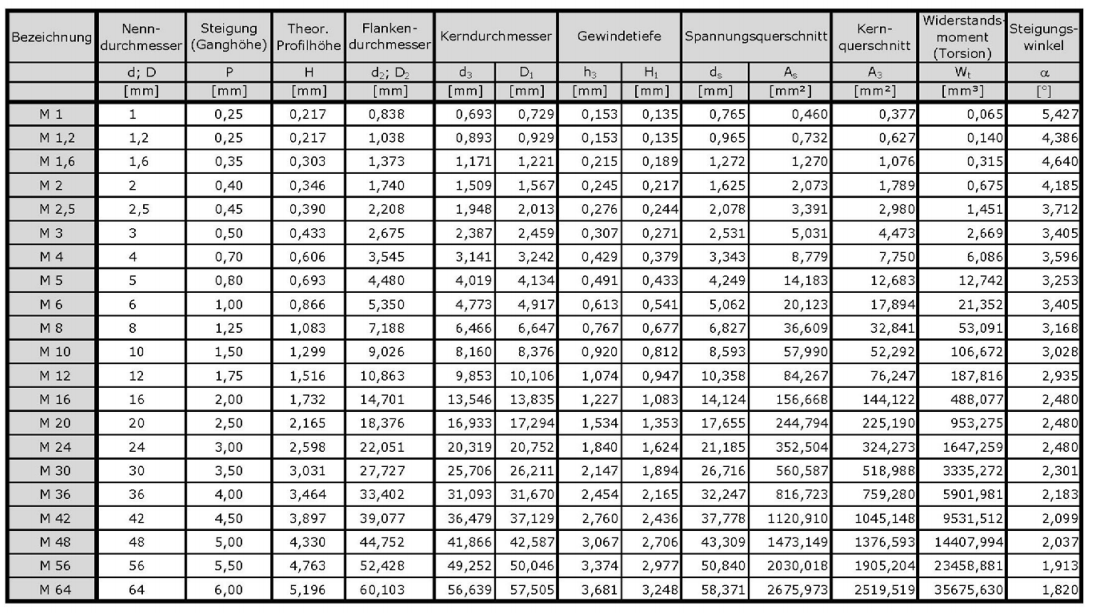
\includegraphics[page=1, scale=0.7, angle=90]{Anhang/Gewindetabelle.png}	
	\end{center}
\end{figure}

\clearpage

\section*{Technische Zeichnungen}

Im folgenden sind technische Zeichnungen zu allen Teilen aufgeführt, die für den Aufbau des designten Wirbelbetts benötigt werden.


\captionsetup{listof=false}

\begin{figure}  
	\captionabove{Halter oben 5mm}
	\includegraphics[page=1, scale=0.9, angle=90]{Anhang/Halter_oben_5mm.pdf}
\end{figure}

\begin{figure}  
	\captionabove{Halter oben 20mm}
	\includegraphics[page=1, scale=0.8, angle=90]{Anhang/Halter_oben_20mm.pdf}
\end{figure}

\begin{figure}  
	\captionabove{Halter oben 30mm}
	\includegraphics[page=1, scale=0.8, angle=90]{Anhang/Halter_oben_30mm.pdf}
\end{figure}

\begin{figure}  
	\captionabove{Halter oben 40mm}
	\includegraphics[page=1, scale=0.7, angle=90]{Anhang/Halter_oben_40mm_Blatt__1.pdf}
\end{figure}

\begin{figure}  
	\includegraphics[page=1, scale=0.8, angle=90]{Anhang/Halter_oben_40mm_Blatt__2.pdf}
\end{figure}

\begin{figure}  
	\captionabove{Schanierarm}
	\includegraphics[page=1, scale=0.7, angle=90]{Anhang/Schanierarm.pdf}
\end{figure}

\begin{figure}  
	\captionabove{Anschlusszylinder}
	\includegraphics[page=1, scale=0.8, angle=90]{Anhang/Anschlusszylinder_Blatt__1.pdf}
\end{figure}

\begin{figure}  
	\includegraphics[page=1, scale=0.8, angle=90]{Anhang/Anschlusszylinder_Blatt__2.pdf}
\end{figure}

\begin{figure}  
	\captionabove{Trichter 5mm}
	\includegraphics[page=1, scale=0.8, angle=90]{Anhang/Trichter_5mm.pdf}
\end{figure}

\begin{figure} 
	\captionabove{Trichter 20mm} 
	\includegraphics[page=1, scale=0.8, angle=90]{Anhang/Trichter_20mm.pdf}
\end{figure}

\begin{figure}
	\captionabove{Trichter 30mm}  
	\includegraphics[page=1, scale=0.8, angle=90]{Anhang/Trichter_30mm.pdf}
\end{figure}

\begin{figure}  
	\captionabove{Trichter 40mm}
	\includegraphics[page=1, scale=0.8, angle=90]{Anhang/Trichter_40mm.pdf}
\end{figure}

\begin{figure}  
	\captionabove{Swagelokrohrhalter}
	\includegraphics[page=1, scale=0.8, angle=90]{Anhang/Swagelokrohrhalter.pdf}
\end{figure}

\begin{figure}  
	\captionabove{Swagelokrohrhalter 2}
	\includegraphics[page=1, scale=0.8, angle=90]{Anhang/Swagelokrohrhalter2.pdf}
\end{figure}

\begin{figure}  
	\captionabove{Befeuchter Spirale}
	\includegraphics[page=1, scale=0.8, angle=90]{Anhang/Spirale_Befeuchter.pdf}
\end{figure}

\clearpage


\section*{Angebote und Rechnungen}

\includepdf[pages={1-2}, scale=0.9]{Anhang/Brooks_Flowcontroller_Angebot.pdf}

\includepdf[pages={1-2}, scale=0.9]{Anhang/O-Ringe1_Angebot.pdf}

\includepdf[pages={1-2}, scale=0.9]{Anhang/O-Ringe2_Angebot.pdf}

\includepdf[pages={1}, scale=0.9]{Anhang/Rechnung_Amazon_Nylonnetz.pdf}
